\documentclass[12pt, twoside]{book}
\usepackage[a4paper,width=150mm,top=25mm,bottom=25mm,bindingoffset=6mm]{geometry}
\usepackage[utf8]{inputenc}
% \usepackage[T1]{fontenc}
\usepackage[italian]{babel}
\usepackage{caption}
\usepackage{forest}
\usepackage{fancyhdr}
\usepackage{newlfont}
\usepackage{float}
\usepackage{xcolor}
\usepackage[nottoc]{tocbibind}
\usepackage{emptypage}
\usepackage{titlesec}
\usepackage[T1]{fontenc}
\usepackage{blindtext, array}
\usepackage[sorting=none,backend=bibtex]{biblatex}
\usepackage{csquotes}
\usepackage{pdfpages}
\usepackage{listings}
\usepackage{amsmath}
\usepackage[cache=false]{minted}
\usepackage{setspace}
\usepackage[hidelinks]{hyperref}
\usepackage{outline}
\usepackage{enumitem}
\setlist{nosep}

% \usepackage{ifxetex}
\usepackage{ifluatex}
\newif\ifxetexorluatex % a new conditional starts as false
\ifnum 0\ifxetex 1\fi\ifluatex 1\fi>0
   \xetexorluatextrue
\fi

\ifxetexorluatex
  \usepackage{fontspec}
\else
  \usepackage[T1]{fontenc}
  \usepackage[utf8]{inputenc}
  \usepackage[lighttt]{lmodern}
\fi

\usepackage{textcomp}
\usepackage{xcolor}
\usepackage{listings}
\usepackage{upquote}

\definecolor{keyword}{HTML}{2771a3}
\definecolor{pattern}{HTML}{b53c2f}
\definecolor{string}{HTML}{be681c}
\definecolor{relation}{HTML}{7e4894}
\definecolor{variable}{HTML}{107762}
\definecolor{comment}{HTML}{8d9094}

\lstset{
	numbers=none,
	stepnumber=1,
	numbersep=5pt,
	basicstyle=\small\ttfamily,
	keywordstyle=\color{keyword}\bfseries\ttfamily,
	commentstyle=\color{comment}\ttfamily,
	stringstyle=\color{string}\ttfamily,
	identifierstyle=,
	showstringspaces=false,
	aboveskip=3pt,
	belowskip=3pt,
	columns=flexible,
	keepspaces=true,
	breaklines=true,	
	captionpos=b,
	tabsize=2,
	frame=none,
}

\lstset{upquote=true}

\lstdefinelanguage{cypher}
{
	morekeywords={
		MATCH, OPTIONAL, WHERE, NOT, AND, OR, XOR, RETURN, DISTINCT, ORDER, BY, ASC, ASCENDING, DESC, DESCENDING, UNWIND, AS, UNION, WITH, ALL, CREATE, DELETE, DETACH, REMOVE, SET, MERGE, SET, SKIP, LIMIT, IN, CASE, WHEN, THEN, ELSE, END,
		INDEX, DROP, UNIQUE, CONSTRAINT, EXPLAIN, PROFILE, START,
	}
}


\newcommand{\mycdots}{\cdot\!\cdot\!\cdot}
\lstset{language=cypher,
	literate=*
	{...}{$\mycdots$}{1}
	{theta}{$\theta$}{1}
}


\definecolor{folderbg}{RGB}{124,166,198}
\definecolor{folderborder}{RGB}{110,144,169}

\def\Size{4pt}
\tikzset{
    folder/.pic={
            \filldraw[draw=folderborder,top color=folderbg!50,bottom color=folderbg]
            (-1.05*\Size,0.2\Size+5pt) rectangle ++(.75*\Size,-0.2\Size-5pt);
            \filldraw[draw=folderborder,top color=folderbg!50,bottom color=folderbg]
            (-1.15*\Size,-\Size) rectangle (1.15*\Size,\Size);
        }
}

% Stile di pagina
% \pagestyle{fancy}
\usemintedstyle{colorful}

\definecolor{lightgray}{gray}{0.95}

% Stile dei titoli dei capitoli
\definecolor{gray75}{gray}{0.75}
\newcommand{\hsp}{\hspace{20pt}}
\titleformat{\chapter}[hang]
{\Huge\bfseries}
{\thechapter\hsp\textcolor{gray75}{|}\hsp}
{0pt}
{\Huge\bfseries}

% Bibliografia
\addbibresource{./biblio/biblio.bib}

\onehalfspacing
\begin{document}

% 
\includepdf{./frontespizio/frontespizio.pdf}
\documentclass[12pt,a4paper]{report}
\usepackage[italian]{babel}
\usepackage{newlfont}
\textwidth=450pt\oddsidemargin=0pt

\begin{document}
\begin{titlepage}

    \begin{center}
        {{\Large{\textsc{Alma Mater Studiorum $\cdot$ Universit\`a di Bologna}}}}
        \rule[0.1cm]{15.8cm}{0.1mm}
        \rule[0.5cm]{15.8cm}{0.6mm}
        \\\vspace{3mm}

        {\small{\bf Scuola di Ingegneria e Architettura \\
                Dipartimento di Informatica $\cdot$ Scienza e Ingegneria $\cdot$ DISI\\
                Corso di Laurea in Ingegneria Informatica}}


    \end{center}

    \vspace{23mm}

    \begin{center}{
            \large \bf DATABASE A GRAFI PER SISTEMA DI CONTROLLO DELLE VERSIONI\par
        }\end{center}

    \vspace{40mm} \par \noindent

    \begin{minipage}[t]{0.47\textwidth}{
        \large{
        Relatore:
        \vspace{2mm}\\{
        \bf Prof. Paolo Ciaccia
        }
        }
        }
    \end{minipage}
    %
    \hfill
    %
    \begin{minipage}[t]{0.47\textwidth}\raggedleft{
            {\large{Presentata da:
                        \vspace{2mm}\\
                        \bf Riccardo Barbieri}}}
    \end{minipage}

    \vspace{40mm}

    \begin{center}
        Anno Accademico 2021/2022
    \end{center}

\end{titlepage}
\end{document}


\phantomsection
\listoffigures


\tableofcontents

\chapter*{Introduzione}
\label{chap:intro}
\addcontentsline{toc}{chapter}{Introduzione}
Un VCS (Version Control System) è un tipo di sistema utile a gestire le versioni di un progetto.
Nell'ambito dello sviluppo di progetti software, la funzionalità principale di un sistema di 
questo tipo è la possibilità di tenere traccia delle modifiche apportate al codice sorgente, ai file
di documentazione e ad altri contenuti di un progetto.\\
Senza l'utilizzo di un VCS, gli sviluppatori di un progetto potrebbero semplicemente mantenere diverse 
copie dei contenuti, classificandole a seconda della versione e delle modifiche apportate da una 
versione all'altra; un approccio simile tuttavia diventa ingestibile per progetti di grandi dimensioni,
in quanto si verrebbero a creare molteplici copie di file uguali o molto simili tra di loro.

In questo lavoro di tesi verrà illustrato e discusso il processo di sviluppo di un rudimentale VCS, 
chiamato GGit (ispirato a Git), basato su un database a grafi e implementato come una applicazione CLI
in Python 3.10.

I database a grafi sono database che fanno uso di strutture a grafi per immagazzinare informazioni.
Questo tipo di struttura è composta da due elementi fondamentali, nodi (o vertici) e archi, applicando
all'ambito dei database, i nodi sono utilizzati per rappresentare le entità, mentre gli archi
rappresentano le relazioni tra le entità.

Una delle proprietà più vantaggiose dei database a grafi utilizzati per questo progetto, ovvero 
LPG o labeled-property graph, consiste nel fatto che il tempo di attraversamento di un grafo 
è costante\cite{traversaltime}.

\chapter{Scelte progettuali}
\label{chap:scelte_progettuali}
Analizzando la scelta dei tool disponibili per il versioning, si evince che Git è il VCS più diffuso e più utilizzato\cite{gitmostused} dagli sviluppatori, è facile da utilizzare per i principianti ma allo stesso tempo supporta funzionalità avanzate per gli utenti più esperti. Per questo motivo si è deciso di ispirarsi al suo funzionamento per la realizzazione di \texttt{GGit}, mantenendo l'interfaccia utente esposta da Git, seppur in forma ridotta, per creare un'esperienza di utilizzo familiare.
\section{Strutture dati di GGit}
\label{sec:strutture_dati}
Git è nato come un semplice content-addressable filesystem, ovvero un sistema di storage basato su una relazione chiave-valore, nel quale è possibile archiviare qualsiasi tipo di contenuto digitale. Essenzialmente, l'azione di base che Git esegue è quella di memorizzare i contenuti di un file associandoli ad un hash calcolato su di essi: questa è la chiave che può essere utilizzata per accedere ai dati salvati.

L'hash di ogni oggetto (nomenclatura utilizzata per file e altre entità descritte in seguito), è calcolato usando l'algoritmo SHA-1, una funzione di hashing che genera un hash di 20 byte.
Pur essendo un algoritmo di hashing crittografico, SHA-1 non è sicuro, in quanto è stato provato che è possibile generare collisioni\cite{sha1collision} (ovvero due input che generano lo stesso hash).
Tuttavia, per l'utilizzo al quale è destinato all'interno di un VCS (cioè identificare univocamente il contenuto di un file) la complessità di SHA-1 è sufficiente, in quanto, nel peggior caso trovato, è stato necessario effettuare $2^{61}$ operazioni per ottenere una collisione\cite{collisionprob}.

Git si basa su 5 tipi di oggetti:
\begin{itemize}
    \item blob: oggetti che rappresentano un file;
    \item tree: oggetti che rappresentano una directory;
    \item commit: oggetti che pongono un particolare tree (la root directory) nella storia della repository, associando un commit padre, un timestamp e un messaggio che descrive le modifiche apportate;
    \item tag: un container che riferisce un altro oggetto, usato prevalentemente per dare un nome a un commit;
    \item packfile: una versione compressa di una serie di oggetti.
\end{itemize}
Il contenuto che verrà dato come input alla funzione di hash sarà una stringa che racchiude le caratteristiche dello specifico oggetto, fattore che aiuta a ridurre ulteriormente la probabilità di collisioni.

Si è deciso di strutturare il modello del dominio di GGit considerando i primi tre tipi di oggetti: blob, tree e commit.
Di seguito viene illustrato come vengono calcolati gli hash di ogni tipo di oggetto.

\subsection{Blob}
Un file è rappresentato da un blob, per calcolarne l'hash si considera la caratteristica principale, ovvero il suo contenuto, che viene considerato in byte sia per file in puro testo ASCII che binari.
Viene poi calcolata la lunghezza in byte del contenuto e il valore risultante viene concatenato con la stringa \texttt{"blob "}, seguita da un carattere NULL il tutto seguito dal contenuto del file:
\begin{minted}[bgcolor=lightgray,framesep=2mm,baselinestretch=1.2,fontsize=\footnotesize]{bash}
blob <file_length>\0<file_content>
\end{minted}
\subsection{Tree}
Un tree è essenzialmente una collezione di blob e tree, la funzione di un tree è associare a blob e tree un nome e una stringa che esprime i permessi sul file.


I permessi sono espressi in modo analogo alla modalità utilizzata dai sistemi UNIX, ovvero tre caratteri ottali che indicano i permessi di lettura, scrittura e esecuzione per il proprietario, il gruppo e gli altri utenti, una cifra ottale che rappresenterebbe i bit setuid, setgid e sticky (ignorati da Git) e altri tre caratteri ottali che indicano la POSIX mode\cite{gitmodes} dell'oggetto:
\begin{itemize}
    \item 04 per directory;
    \item 10 per file regolari;
    \item 12 per link simbolico;
    \item 16 per Git link o sottomoduli, non presente tra le classiche POSIX modes (non supportati da GGit).
\end{itemize}
L'hash di un tree viene calcolato in modo analogo a quello di un blob:
\begin{minted}[bgcolor=lightgray,framesep=2mm,baselinestretch=1.2,fontsize=\footnotesize]{bash}
tree <tree_length>\0<tree_content>
\end{minted}
dove \texttt{tree\_length} è la lunghezza in byte del \texttt{tree\_content}, che è una lista di oggetti, in ordine alfabetico per nome, nel seguente formato:
\begin{minted}[bgcolor=lightgray,framesep=2mm,baselinestretch=1.2,fontsize=\footnotesize]{bash}
<object_mode> <object_name>\0<object_hash>
\end{minted}
La stringa \texttt{object\_name} è il nome del file o directory e \text{object\_hash} l'hash dell'oggetto corrispondente.
La \texttt{object\_mode} è la stringa di sei caratteri ottali che identifica il tipo e i permessi dell'oggetto descritta in precedenza, questa stringa in GGit può assumere i seguenti valori:
\begin{itemize}
    \item 100644 per file regolari;
    \item 100755 per file eseguibili;
    \item 040000 per directory (altri tree);
    \item 120000 per link simbolici,
\end{itemize}
nel caso in cui la stringa abbia zeri iniziali, questi vengono troncati (regola applicabile soltanto nel caso delle directory).
\subsection{Commit}
La funzione principale di un commit è quella di associare lo stato corrente dell'area di commit a un punto nella storia della repository e facilitare la reperibilità di un particolare stato della repository.
L'area di commit, in GGit chiamata \texttt{stash}, è essenzialmente una lista di file che verranno aggiunti al prossimo commit.
Per calcolare l'hash di un commit si procede in modo analogo a quello degli altri tipi di oggetti:
\begin{minted}[bgcolor=lightgray,framesep=2mm,baselinestretch=1.2,fontsize=\footnotesize]{bash}
commit <commit_length>\0<commit_content>
\end{minted}
dove \texttt{commit\_length} è la lunghezza in byte del \texttt{commit\_content}, che è una stringa formattata come segue:
\begin{minted}[bgcolor=lightgray,framesep=2mm,baselinestretch=1.2,fontsize=\footnotesize]{text}
tree <tree_hash>
parent <parent_hash>
author <author_name> <<author_email>> <author_timestamp> <timezone>
committer <committer_name> <<committer_email>> <committer_timestamp> <timezone>

<commit_message>
\end{minted}
Il \texttt{tree\_hash} è l'hash del tree che rappresenta la root directory dell'area di lavoro, il \texttt{parent\_hash} è l'hash del commit padre, ovvero il commit dal quale è stato creato il commit corrente, se il commit è il primo della storia della repository, questo campo è omesso.
Le due linee successive contengono le informazioni che identificano rispettivamente l'utente che ha implementato le modifiche (author) e l'utente che ha creato il commit (committer). A oggi GGit non supporta la possibilità di applicare patch a commit passati come Git\cite{gitdocsauthcomm}, è però possibile, al momento della creazione del commit, specificare un autore diverso dal committer, per dare credito all'effettivo autore del codice e non solo all'utente che lo ha accettato all'interno della repository.
Infine l'ultima riga è il messaggio associato al commit, stringa che idealmente descrive le modifiche che vengono implementate con il commit.
\section{Database}
\label{sec:database}
I tipi di oggetti in gioco hanno un alto livello di interconnessione tra di loro: ogni commit è relativo a un tree, un tree può contenere molteplici blob e tree e un tree diverso può contenere un sottoinsieme di blob e tree di un altro tree. Data questa caratteristica, si è scelto di utilizzare un database a grafi.

La gamma di diversi tipi di database a grafi è ampia (anche se non come nel caso dei database relazionali); si è scelto di utilizzare per questo progetto Neo4j, un database a grafi scalabile orizzontalmente del quale esiste una community edition totalmente opensource\cite{neo4jgit}. Neo4j è inoltre il database a grafi più utilizzato\cite{db-engines_2022}, con una vasta community di sviluppatori, il che aiuta in fase di sviluppo per trovare soluzioni ad eventuali problemi.

Un'altra caratteristica che ha portato alla scelta di questo particolare database sono i tool a supporto dello sviluppo, come ad esempio Neo4j Desktop o Browser, che espongono una interfaccia grafica intuitiva per eseguire query e visualizzare rappresentazioni grafiche dei grafi risultanti; è disponibile inoltre Neo4j AuraDB che permette di effettuare il deployment di un database a grafi in cloud, permettendo quindi di creare repository condivise senza necessità di gestire infrastrutture server.

\subsection{Sviluppo del modello di dati}
\label{sec:datamodel}
Il modello di dati è stato sviluppato per poter rappresentare in modo completo tutti i tipi di oggetti presenti in GGit e grazie alla caratteristica schema-less dei database a grafi, sarà possibile aggiungere nuovi tipi di oggetti o caratteristiche al modello del dominio senza intaccare maggiormente la struttura preesistente.

Anche se il database scelto è schema-less, è comunque buona pratica definire e documentare in modo preciso il modello dei dati, così da evitare in futuro di fare scelte incompatibili con il modello preesistente.

Per sviluppare il modello dei dati è possibile sfruttare l'approccio "whiteboard", che permette di rappresentare il modello in modo grafico per esprimere ad alto livello le entità e le relazioni in gioco per poi formalizzare la struttura senza dover convertire le decisioni prese in tabelle.
\begin{figure}[H]
    \centering
    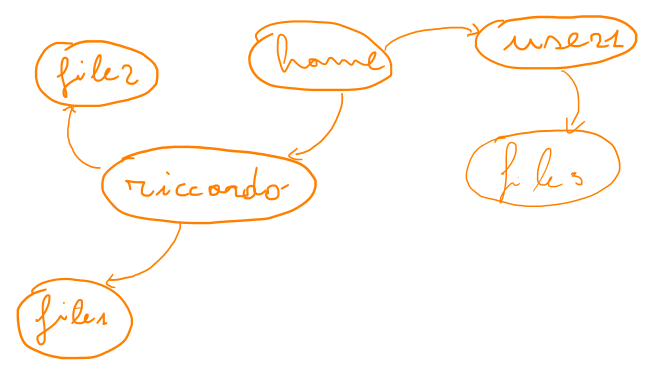
\includegraphics[width=15cm]{./immagini/whiteboard_sketch.png}
    \caption{Whiteboard sketch della struttura di un'ipotetica repository}
\end{figure}
Dopo aver creato il cosiddetto "whiteboard model" si procede alla formalizzazione delle entità e relazioni individuate, etichettando con label le entità e relazioni e associandovi tutte le proprietà.
\begin{figure}[H]
    \centering
    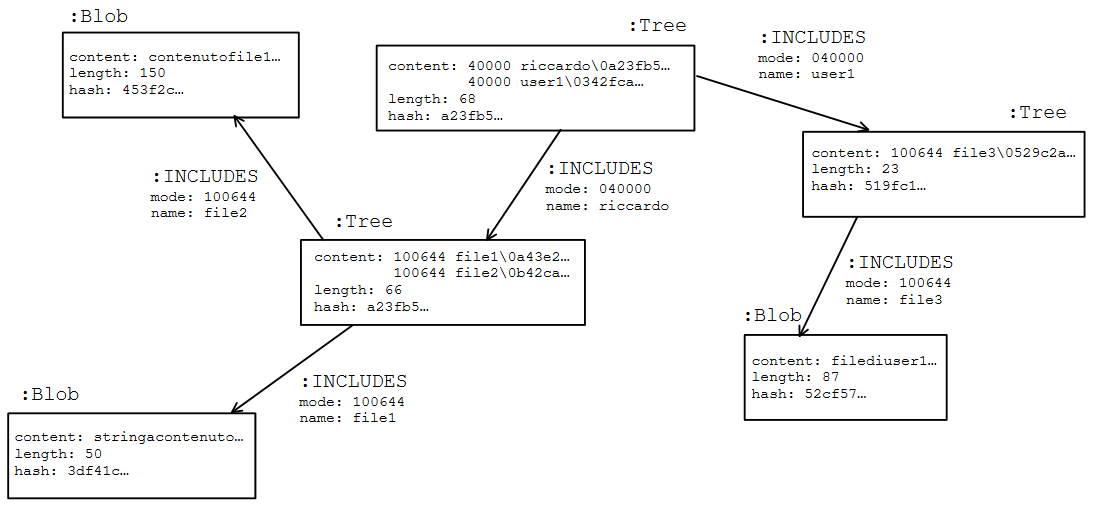
\includegraphics[width=15cm]{./immagini/whiteboard_formal.png}
    \caption{Formalizzazione dello sketch con proprietà e label}
\end{figure}
Come si nota dalla figura precedente si è deciso di assegnare i label (case sensitive) \texttt{:Tree} e \texttt{:Blob} alle rispettive entità, si individuano inoltre le seguenti proprietà per entrambi i tipi di oggetti:
\begin{itemize}
    \item \texttt{hash}: identificatore univoco dell'oggetto, calcolato con l'algoritmo SHA-1;
    \item \texttt{size}: dimensione in byte del contenuto;
    \item \texttt{content}: contenuto dell'oggetto, come descritti sopra.
\end{itemize}

Per quanto riguarda le relazioni, in questo sottoinsieme del modello se ne individua soltanto una: il label \texttt{:INCLUDES} indica che un oggetto ne contiene un altro. Le relazioni sono ordinate e nel caso di \texttt{:INCLUDES} il nodo di partenza è sempre un \texttt{:Tree} e il nodo di arrivo può essere sia un \texttt{:Tree} che un \texttt{:Blob}.
Si denotano inoltre due proprietà per questa relazione:
\begin{itemize}
    \item \texttt{name}: nome del file o della directory;
    \item \texttt{mode}: GGit mode dell'oggetto, può assumere il valore "040000" se il nodo di arrivo ha il label \texttt{:Tree} e i valori {"100644", "100755", "120000"} se il nodo di arrivo ha il label \texttt{:Blob}.
\end{itemize}

È stata fatta la scelta di associare le proprietà \texttt{name} e \texttt{mode} alla relazione e non al nodo in quanto rispecchia correttamente il modello dei dati definito: un oggetto \texttt{blob}, così come un \texttt{tree}, non ha un nome o una mode associati fino al momento in cui viene inserito all'interno di un \texttt{tree}.

Sotto viene mostrato il whiteboard sketch relativo al modello dei \texttt{commit} e degli \texttt{user}, e come possono essere collegati tra di loro:
\begin{figure}[H]
    \centering
    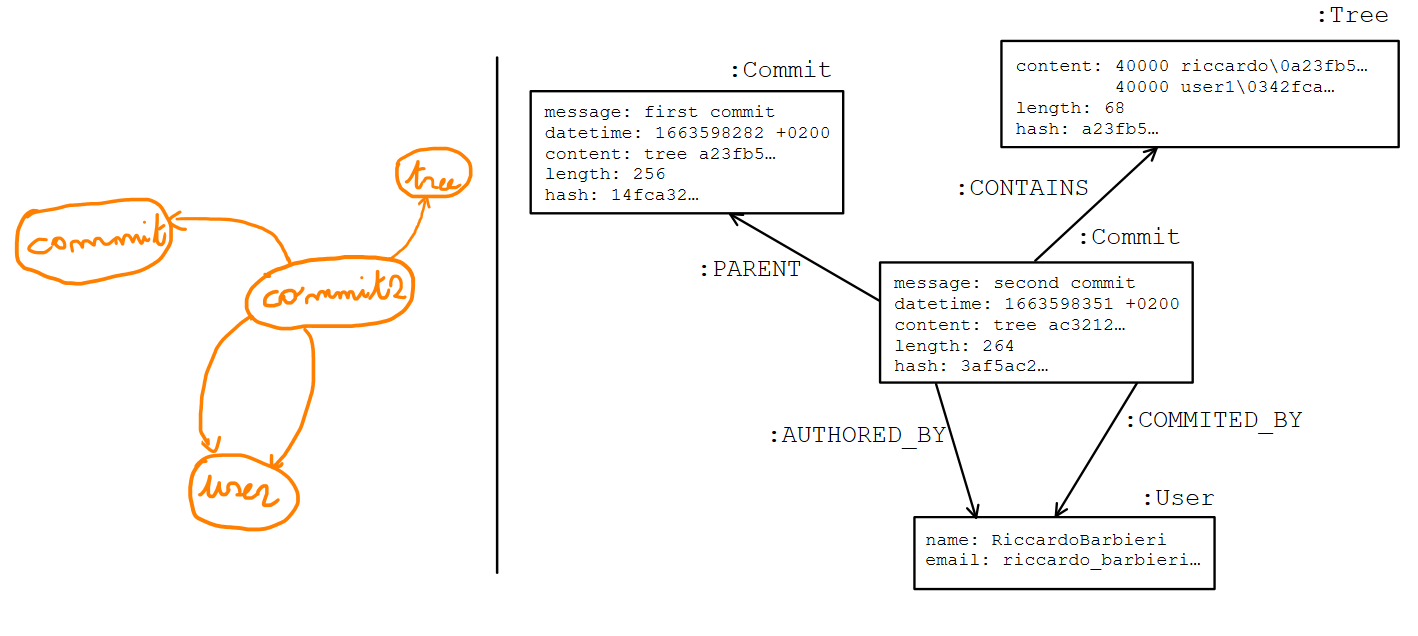
\includegraphics[width=15cm]{./immagini/whiteboard_commit.png}
    \caption{Whiteboard sketch del modello dei commit e degli user}
\end{figure}
In questa sezione del modello si individuano due nuove entità, \texttt{:Commit}, che è identificata dalle seguenti proprietà:
\begin{itemize}
    \item \texttt{message}: messaggio del commit;
    \item \texttt{datetime}: momento di creazione del commit (UNIX timestamp) e fuso orario (in ore dal UTC);
    \item \texttt{content}: stringa che rappresenta il commit (quella che viene data come input all'algoritmo di hashing).
    \item \texttt{length}: lunghezza del content.
    \item \texttt{hash}: identificatore univoco del commit, calcolato come descritto sopra,
\end{itemize}
e \texttt{:User}, identificata dalle seguenti proprietà:
\begin{itemize}
    \item \texttt{name}: nome dell'utente;
    \item \texttt{email}: email dell'utente;
\end{itemize}
Si identificano inoltre nuove relazioni: \texttt{:COMMITTED\_BY} e \texttt{:AUTHORED\_BY} che indicano rispettivamente il committer e l'autore di un commit; \texttt{:PARENT} che parte da un commit e punta al commit padre e infine \texttt{:CONTAINS} che parte da un commit e punta ad un oggetto \texttt{tree} che rappresenta lo stato della repository al momento del commit.

Come dimostrato, il modello whiteboard è estremamente utile per formalizzare le entità e relazioni in gioco e per individuare le proprietà da associare ad esse, data la natura ad alto livello di questo approccio è molto semplice passare da un idea, o uno sketch, a una definizione formale del modello dei dati.
\section{Stato della repository}
\label{sec:stato}
In questa sezione verranno descritte le modalità di gestione dello stato della repository, che comprende la lista dei file cosiddetti "tracked"; la lista dei file "stashed" e la gestione delle differenze dei file dell'ultima versione.

\subsection{Stash e tracking}
\label{subsec:stash}
Una delle funzioni fondamentali che GGit utilizza per tenere traccia della storia di una repository è l'area di \texttt{stash}, questa è l'area che raccoglie la lista dei file che verranno aggiunti al prossimo commit.
Questa area è strettamente legata alla lista dei file tracked, che sono quei file che un qualsiasi punto nella storia della repository sono stati aggiunti all'area di stash.

Si è scelto di mantenere l'area di stash e tracking nella repository stessa, in memoria locale, in modo da evitare di dover sostenere una connessione al database per operazioni che possono essere ripetute frequentemente.

\subsection{Differenze tra versioni di file}
\label{subsec:differenze}
GGit è in grado di riportare quali file sono stati modificati rispetto all'ultima versione, nella versione corrente dell'applicazione questa funzione è utile soltanto ai fini di un particolare comando (descritto successivamente) ma si è deciso di aggiungere questa funzionalità a supporto di future operazioni, come ad esempio la gestione di conflitti durante il merge automatico di versione differenti di uno stesso file.

\section{Gestione del server Neo4j}
Inizialmente si era pensato di includere una distribuzione del server Neo4j all'interno del package dell'applicazione, in modo da non dover richiedere all'utente di installare il server autonomamente, tuttavia si è scelto di istruire l'utente a installare una versione del server Neo4j, la directory dell'installazione andrà poi specificata all'interno di una variabile d'ambiente chiamata \texttt{"NEO4J\_HOME"}, variabile che verrà utilizzata per reperire l'installazione e copiarla all'interno di ciascuna repository; il database copiato viene poi inizializzato.

È stata fatta questa scelta per permettere di utilizzare la versione community del server di Neo4j per repository locali, versione che non permette di creare multipli database associati allo stesso server, è comunque possibile utilizzare una versione enterprise del server, ma richiede configurazione aggiuntiva (discussa nelle \hyperref[sec:impostazioni]{Impostazioni di configurazione}).
Inoltre è possibile connettersi ad un server Neo4j remoto, in questo caso è necessario specificare l'indirizzo del server e le credenziali di accesso attraverso le impostazioni di configurazione.

\section{Interfaccia utente}
\label{sec:interfaccia}
L'interfaccia utente di \texttt{GGit} è ispirata a quella di \texttt{Git}, del quale si è deciso di implementare un sottoinsieme ridotto di comandi, ovvero quelli essenziali al funzionamento di base di un VCS:
\begin{itemize}
    \item \texttt{init};
    \item \texttt{add};
    \item \texttt{mv};
    \item \texttt{rm};
    \item \texttt{commit};
    \item \texttt{status};
    \item \texttt{config};
    \item \texttt{log}.
\end{itemize}

\subsection{Gestione della repository}
Questi sono i comandi per gestire la repository.

\subsubsection{Init}
Il comando \texttt{ggit init} crea una nuova repository, in particolare viene create la directory \texttt{.ggit} all'interno della directory nella quale viene chiamato il comando, si è però deciso di permettere all'utente di specificare la directory da inizializzare con il comando \texttt{ggit init <path>}, in questo modo è possibile creare una repository all'interno di una directory diversa dalla corrente.

Dopo aver creato la directory, vengono inizializzati i file di configurazione e dello stato e vengono impostate alcune configurazioni di base, viene inoltre richiesto interattivamente all'utente di inserire username e email, che verranno utilizzati per i commit.
Viene poi inizializzato lo stato della repository, reperita l'installazione di Neo4j e impostate le impostazioni relative a username, password e nome, versione e posizione del database.

\subsubsection{Config}
Il comando \texttt{ggit config} permette di gestire le impostazioni di configurazione, in particolare è possibile visualizzare le impostazioni correnti, impostare nuove impostazioni e rimuovere impostazioni esistenti.

Questo comando offre i seguenti parametri:
\begin{itemize}
    \item \texttt{-{}-list} per visualizzare tutte le impostazioni correnti;
    \item \texttt{-{}-get <key>} per visualizzare il valore di una impostazione;
    \item \texttt{-{}-set <key> <value>} per impostare il valora di una impostazione, se non esiste viene aggiunta;
    \item \texttt{-{}-unset <key>} per rimuovere una impostazione.
\end{itemize}

\subsection{Gestione dei file}
I seguenti comandi sono disponibili all'utente per modificare lo stato della repository, aggiungendo rimuovendo e spostando file.

Tutti i comandi in questa categoria supportano l'utilizzo da qualsiasi sottodirectory della repository, tenendo conto della relatività degli eventuali path specificati.
\subsubsection{Add}
Il comando \texttt{ggit add} permette di aggiungere un lista di file e/o directory all'area di \texttt{stash} della repository; ogni volta che un file viene aggiunto, viene anche inserito nella lista dei file tracked, nel caso delle directory vengono aggiunti tutti i file contenuti nella directory stessa e in tutte le sottodirectory.

Il comando offre un solo parametro, obbligatorio, che accetta valori multipli sotto forma di lista separata da spazi, questi sono le stringhe che verranno interpretate come path.

\subsubsection{Mv}
Il comando \texttt{ggit mv} permette di spostare un file o una directory da una posizione all'altra, in questo caso il file viene effettivamente spostato nel file system e viene aggiornato il path del file nella lista dei file tracked e dello stash.

Il comando accetta due parametri, obbligatori, che accettano rispettivamente un solo valore che verrà interpretato come path, il primo è il file o la directory di partenza e il secondo la destinazione.

\subsubsection{Rm}
Il comando \texttt{ggit rm} permette di rimuovere un file o una directory, specificati come parametri, dalla lista dei file tracked e dello stash, in questo caso il file viene rimosso dal file system.

Così come il comando \texttt{add}, anche questo comando supporta l'utilizzo di valori multipli, separati da spazi, per specificare più file o directory da rimuovere.

\subsection{Gestione della storia}
\subsubsection{Commit}
Il comando \texttt{ggit commit} permette di creare un nuovo commit partendo dallo stato corrente dello stash della repository.

Inizialmente viene creato un nuovo oggetto tree, partendo dallo stash della repository. Dopodiché vengono interpretate le opzioni passate al comando, in particolare è possibile specificare:
\begin{itemize}
    \item \texttt{-m} o \texttt{-{}-message}: specifica il messaggio del commit;
    \item \texttt{-f} o \texttt{-{}-file}: specifica il nome del file dal quale leggere il messaggio di commit, mutualmente esclusivo con \texttt{-m};
    \item \texttt{-{}-author}: specifica l'autore del commit, nel formato \texttt{nome,email} per effettuare l'override dell'autore di default;
    \item \texttt{-{}-date}: specifica la data, nel formato \texttt{YYYY-MM-DDTHH:mm:SS+HH:mm} per effettuare l'override della data corrente.
\end{itemize}
Dopo aver valutato e interpretato le opzioni, viene recuperato dalle impostazioni di configurazione l'hash dell'ultimo commit, con il quale si ottiene dal database l'oggetto commit associato che viene assegnato al nuovo commit, se questa impostazione è vuota o non presente, significa che il commit che viene effettuato è il primo e non necessita un parent.

Infine viene effettivamente aggiunto il commit al database, aggiornata l'impostazione relativa all'ultimo commit e viene svuotato lo stash.

\subsection{Visualizzazione dello stato}
\subsubsection{Status}
Il comando \texttt{ggit status} permette di visualizzare un riassunto dello stato corrente della directory, in particolare vengono mostrate tre liste di file.
La prima lista elenca i file che sono al momento nell'area di \texttt{stash} e quindi verranno aggiunti al prossimo commit.
La seconda lista mostra i file che sono stati modificati rispetto al commit precedente, sono stati aggiunti, a un certo punto nella storia della repository, all'area di \texttt{tracking} e non sono ancora nell'area di \texttt{stash}. Infine la terza lista contiene i file che sono stati creati ma non sono mai stati aggiunti all'area di \texttt{stash} e quindi non sono ancora nel tracking della repository.

\subsubsection{Log}
Il comando \texttt{ggit log} permette di visualizzare lo storico dei commit della repository, stampa una lista dei commit più recenti, mostrando il loro hash, l'autore, la data di creazione e il messaggio di commit.

Il comando supporta una opzione \texttt{-d} o \texttt{-{}-depth} che permette di specificare il numero di commit da visualizzare, il valore di default è impostato a 5.

\section{Impostazioni di configurazione}
\label{sec:impostazioni}
Le impostazioni di configurazione sono una serie di entry chiave-valore, vengono utilizzate dall'applicazione per salvare e ottenere informazioni relative alla configurazione della repository e del database.

Tutte queste impostazioni possono essere aggiunte o modificate manualmente attraverso il comando \texttt{ggit config}.

\subsection{Configurazione della repository}
Alla versione corrente, le impostazioni di configurazione della repository sono le seguenti:
\begin{itemize}
    \item \texttt{"repository.path"}: path che punta alla root directory della repository;
    \item \texttt{"HEAD"}: contiene l'hash dell'ultimo commit effettuato, se non è presente o è impostato a \texttt{"None"} significa che non è ancora stato effettuato nessun commit;
    \item \texttt{"user.name"} e \texttt{"user.email"}: nome dell'utente e email utilizzati per i commit.
\end{itemize}

\subsection{Configurazione del database}
\begin{itemize}
    \item \texttt{"database.username"} e \texttt{"database.password"}, che contengono le credenziali di accesso al database di default;
    \item \texttt{"database.name"}, contiene il nome di default del database nella community edition;
    \item \texttt{"database.path"}, salva il path alla directory di installazione di Neo4j, ottenuto tramite la variabile d'ambiente \texttt{"NEO4J\_HOME"}.
\end{itemize}

Le impostazioni del database vengono inizializzate automaticamente ai valori utili per la community edition, per utilizzarne una enterprise è necessario modificare manualmente le variabile\texttt{"database.username"} e \texttt{"database.password"} con le credenziali personalizzate del database, mentre la variabile \texttt{"database.name"} deve essere impostata al nome del database che si vuole utilizzare.
\chapter{Implementazione}
In questo capitolo verrà illustrato il processo di implementazione di \texttt{GGit}, facendo riferimento alle scelte progettuali discusse e ponendo particolare attenzione alle problematiche riscontrate durante lo sviluppo.

Come già accennato, si è scelto di sviluppare \texttt{GGit} utilizzando Python 3.10, decisione derivata dal fatto che Python è un linguaggio molto flessibile e che permette uno sviluppo veloce sin dai primi passi di un progetto; un altro vantaggio non indifferente è la disponibilità di una quantità disarmante di librerie potenti e ben documentate, che semplificano molto alcune fasi dello sviluppo.

Si inizierà con una breve descrizione delle decisioni prese in merito alla suddivisione in package del codice, per poi passare a una analisi più approfondita delle porzioni di codice più interessanti per ogni modulo. Per precisare, in Python, per package si intende un contenitore per moduli e sub-package (solitamente una directory), mentre un modulo è semplicemente un file che contiene codice Python.

\subsubsection{Suddivisione in package}



\begin{forest}
    for tree={
    font=\ttfamily,
    grow'=0,
    child anchor=west,
    parent anchor=south,
    anchor=west,
    calign=first,
    inner xsep=7pt,
    edge path={
            \noexpand\path [draw, \forestoption{edge}]
            (!u.south west) +(7.5pt,0) |- (.child anchor) pic {folder} \forestoption{edge label};
        },
    % style for your file node 
    file/.style={edge path={\noexpand\path [draw, \forestoption{edge}]
                    (!u.south west) +(7.5pt,0) |- (.child anchor) \forestoption{edge label};},
            inner xsep=2pt,font=\small\ttfamily
        },
    before typesetting nodes={
            if n=1
                {insert before={[,phantom]}}
                {}
        },
    fit=band,
    before computing xy={l=15pt},
    }
    [ggit
        [app]
        [database]
        [entities]
        [exceptions]
        [git\_utils
            [git\_connector]
            [model]
        ]
        [handlers]
        [managers]
        [test]
        [utils]
    ]
\end{forest}

La figura sopra mostra la struttura di package adottata, si evidenziano particolarmente le cartelle \texttt{database}, \texttt{entities}, \texttt{handlers} e \texttt{managers}, che contengono i moduli più importanti per il funzionamento di \texttt{GGit}.

\section{Entità}

Il package \texttt{entities} contiene i moduli che espongono le classi che rappresentano le entità del dominio di \texttt{GGit}. In particolare, si trovano le classi \texttt{Blob}, \texttt{Commit}, \texttt{Tree} e \texttt{User}. Ogni classe è implementata in un file separato.



\begin{forest}
    for tree={
    font=\ttfamily,
    grow'=0,
    child anchor=west,
    parent anchor=south,
    anchor=west,
    calign=first,
    inner xsep=7pt,
    edge path={
            \noexpand\path [draw, \forestoption{edge}]
            (!u.south west) +(7.5pt,0) |- (.child anchor) pic {folder} \forestoption{edge label};
        },
    % style for your file node 
    file/.style={edge path={\noexpand\path [draw, \forestoption{edge}]
                    (!u.south west) +(7.5pt,0) |- (.child anchor) \forestoption{edge label};},
            inner xsep=2pt,font=\small\ttfamily
        },
    before typesetting nodes={
            if n=1
                {insert before={[,phantom]}}
                {}
        },
    fit=band,
    before computing xy={l=15pt},
    }
    [ggit
        [...]
        [entities
                [blob.py, file
                ]
                [commit.py, file
                ]
                [tree.py, file
                ]
                [user.py, file
                ]
        ]
        [...]
    ]
\end{forest}

La classe \texttt{ggit.entities.user.User} contiene gli attributi \texttt{name} e \texttt{email} e espone metodi accessor tramite l'uso del docoratore \texttt{property}.

Le classi 
\begin{itemize}
    \itemsep0em
    \item \texttt{ggit.entities.blob.Blob};
    \item \texttt{ggit.entities.tree.Tree};
    \item \texttt{ggit.entities.commit.Commit};
\end{itemize}
espongono metodi per ottenere l'hash dell'oggetto che rappresentano, così come altri metodi per accedere alle informazioni in esse contenuti (contenuto del file per i blob, autore, committer, data etc. per i commit etc.).

Le proprietà calcolate, come il content per tree e commit o la sua lunghezza, sono state progettate per non essere modificate dall'utente, quindi non è stata implementata la funzione setter decorata con \texttt{\{attribute\}.setter}

\section{Database}

Le classi che governano l'interazione con il database sono contenute nei moduli all'interno del package \texttt{database}.
\vspace{15pt}


\begin{forest}
    for tree={
    font=\ttfamily,
    grow'=0,
    child anchor=west,
    parent anchor=south,
    anchor=west,
    calign=first,
    inner xsep=7pt,
    edge path={
            \noexpand\path [draw, \forestoption{edge}]
            (!u.south west) +(7.5pt,0) |- (.child anchor) pic {folder} \forestoption{edge label};
        },
    % style for your file node 
    file/.style={edge path={\noexpand\path [draw, \forestoption{edge}]
                    (!u.south west) +(7.5pt,0) |- (.child anchor) \forestoption{edge label};},
            inner xsep=2pt,font=\small\ttfamily
        },
    before typesetting nodes={
            if n=1
                {insert before={[,phantom]}}
                {}
        },
    fit=band,
    before computing xy={l=15pt},
    }
    [ggit
        [...]
        [database
                [blob\_repository.py, file
                ]
                [commit\_repository.py, file
                ]
                [data\_source.py, file
                ]
                [tree\_repository.py, file
                ]
                [user\_repository.py, file
                ]
        ]
        [...]
    ]
\end{forest}

\subsection{Connessione al database}

Le connessioni al database sono gestite attraverso l'utilizzo della classe DataSource, contenuta nel modulo \texttt{ggit.database.data\_source}.

Un oggetto di questa classe, quando inizializzato, ottiene dalle impostazioni di configurazione le credenziali del database e salva come suo attributo il driver di connessione, inizializzandolo con l'uri fornito e le credenziali ottenute. L'uri del database può essere passato come parametro all'inizializzazione, se non viene specificato viene utilizzato il valore di default \texttt{"bolt://localhost:7687"}.

La classe espone il metodo \texttt{new\_session()}, creato per restituire un oggetto di tipo \texttt{neo4j.Session} legato al driver creato all'inizializzazione, che può essere utilizzato per interagire con il database; l'utilizzo consigliato di questo metodo è insieme allo statement \texttt{with} per creare un context manager che si occupa di chiudere correttamente la sessione una volta terminate le operazioni.
È inoltre esposto il metodo \texttt{close()}, che chiude la connessione al database insieme a tutte le sessioni associate.

Questa classe è stata implementata come singleton tramite l'uso di una metaclass chiamata \texttt{SingletonMeta} (dettagliata in seguito), in modo da utilizzare lo stesso driver durante una singola esecuzione per semplificare la gestione delle sessioni.

\subsection{Mapping entità database}
Per mappare le entità in gioco al database si utilizza una metodologia CRUD (Create, Read, Update, Delete) senza però implementare i metodi di Update, dato che nel VCS non è prevista la modifica di un commit, o dei dati ad esso associati, una volta creato.

Per ogni entità è stata implementata una classe "repository", che espone i metodi necessari per aggiungere, rimuovere e ottenere uno o tutti gli oggetti di quel tipo dal database:
\begin{itemize}
    \item \texttt{add\_\{entity\}} per aggiungere un oggetto nel database;
    \item \texttt{delete\_\{entity\}} per rimuovere un oggetto dal database;
    \item \texttt{get\_\{entity\}} per ottenere un oggetto dal database;
    \item \texttt{get\_all\_\{entity\}} per ottenere tutti gli oggetti di un certo tipo dal database.
\end{itemize}

Queste classi fanno uso della classe \texttt{ggit.database.data\_source.DataSource} per ottenere una sessione con il database e per eseguire le query scritte in Cypher, linguaggio di query di Neo4j.

Cypher è un linguaggio progettato per essere espressivo ed efficiente, permette di esprimere con una sintassi concisa query  anche molto complesse, permette quindi di concentrare l'attenzione sul dominio in considerazione.
inizialmente è nato come linguaggio ad uso esclusivo dei database Neo4j ma nel 2015 è stato scelto come standard per il progetto openCypher\cite{opencypher}, che mira a creare un linguaggio di query comune a tutti i database a grafi.

Di seguito verranno illustrate alcune delle query e modalità di creazione delle entità nel database.

\subsubsection{Gestione di blob e utenti}
Le repository che si occupano della gestione dei blob sono le più semplici, in quanto quando vengono create o eliminate non devono prendersi cura delle relazioni con gli altri oggetti, compito lasciato alle repository delle entità composte.

Esempio di query per creare un oggetto blob:
\begin{minted}[bgcolor=lightgray,framesep=2mm,baselinestretch=1.2,fontsize=\footnotesize]{cypher}
MERGE (b:Blob {id: $blob_id, content: $content})
\end{minted}
Questa query è composta da due sezioni principali: il pattern che segue la parola \texttt{MERGE} e la clausola \texttt{MERGE} che indica come comportarsi con il pattern specificato.

La keyword \texttt{MERGE} indica che se il pattern specificato non è presente nel database, deve essere creato, è anche possibile usarla insieme alle clausole \texttt{ON MATCH} e \texttt{ON CREATE} per specificare come comportarsi nel caso in cui il pattern sia già presente nel database o se deve essere creato, tuttavia in questa query non tornano utili. 

La sintassi dei pattern è progettata per essere simile a come si disegnerebbe un grafo su una lavagna: cerchi per i nodi e freccie per i collegamenti.

Un altro componente della query sono i parametri, indicati con il simbolo \texttt{\$}, che vengono sostituiti con i valori passati come argomento alla funzione che esegue la query.

Per la gestione degli user e dei blob vengono eseguite transazioni autogestite, attraverso l'uso del metodo \texttt{neo4j.Session.run()} che permette di eseguire una query, impostandone opportunamente i parametri, e effettuare automatica il rollback in caso di errore.

\subsubsection{Gestione di commit e tree}
Le repository che si occupano della gestione dei commit e dei tree sono più complesse, in quanto devono creare anche i nodi relativi agli oggetti che li compongono e le relazioni tra di essi, per questo motivo vengono utilizzate transazioni esplicite, che permettono di gestire manualmente il commit o il rollback delle operazioni: in caso di una qualsiasi eccezione durante l'esecuzione delle query per inserire un oggetto complesso, viene effettuato il rollback.

Il metodo \texttt{add\_tree()}, utilizzato per creare un nuovo oggetto tree nel database, come prima cosa crea il nodo principale che rappresenta il tree, si itera poi sulla lista di item contenuti nel tree, creando opportunamente blob attraverso una istanza di \texttt{BlobRepository} e subtree usando il metodo stesso in modo ricorsivo.

Esempio di query utilizzate per creare la relazione tra un tree e un suo subtree:
\begin{minted}[bgcolor=lightgray,framesep=2mm,baselinestretch=1.2,fontsize=\footnotesize]{cypher}
MATCH (t:Tree {hash: $hash}) MATCH (t2:Tree {hash: $hash2})
MERGE (t)-[:INCLUDES {mode: $mode, name: $name}]->(t2)
\end{minted}
Inizialmente vengono identificati i due tree tramite il loro hash nelle clausole \texttt{MATCH}, e successivamente viene utilizzata una \texttt{MERGE} per creare la relazione.

Altre due query interessanti nell'ambito dei tree sono quella per cancellare un tree e per crearne uno nuovo.
\begin{minted}[bgcolor=lightgray,framesep=2mm,baselinestretch=1.2,fontsize=\footnotesize]{cypher}
MATCH (tree:Tree {hash: $hash})-[r*1..]->(n)
DETACH DELETE tree, n
\end{minted}
Con questa query viene cancellato un tree: il pattern identifica il tree principale, tutti i percorsi, di lunghezza almeno 1 (sintassi \texttt{r*1..}), in uscita verso un qualsiasi nodo e i nodi terminali, viene poi utilizzata la clausola \texttt{DETACH DELETE} per eliminare i nodi identificati e tutte le relazioni che li collegano.
\begin{minted}[bgcolor=lightgray,framesep=2mm,baselinestretch=1.2,fontsize=\footnotesize]{cypher}
MATCH relation = (tree:Tree {hash: $hash})-[:INCLUDES*1..]->(item)
RETURN tree, relation, item
\end{minted}
Questa query, eseguita dal metodo \texttt{get\_tree()}, identifica tutti i percorsi composti da relazioni di tipo \texttt{:INCLUDES} di lunghezza almeno 1 in uscita dal tree e tutti i nodi terminali e li restituisce come risultato.
Il risultato viene poi utilizzato dal metodo, sotto forma di oggetto \texttt{neo4j.Graph}, per ricostruire l'entità tree.

L'oggetto \texttt{neo4j.Graph} è una funzionalità sperimentale del driver Neo4j per Python che permette di rappresentare un grafo come un oggetto container di oggetti \texttt{neo4j.Node} e \texttt{neo4j.Relationship}, oggetto che viene passato come parametro alla funzione di utility \texttt{parse\_tree()} che si occupa di ricostruire l'entità tree.
\\~\\
Per creare nuovi commit invece, si procede con l'apposito metodo \texttt{add\_commit()} che si assicura, tramite una \texttt{UserRepository}, che esistano gli utenti necessari, per poi passare alla creazione del nodo commit, legandolo contemporaneamente ad autore e committer.
Se il commit ha un parent, viene creata la relazione tra i due commit, viene successivamente aggiunto il main tree del commit usando una \texttt{TreeRepository}, infine viene creata la relazione \texttt{:CONTAINS} tra il commit e il main tree.

L'eliminazione di un commit non è ancora supportata dal sistema, ma è comunque implementato il metodo utile a cancellare il nodo e tutte le relazioni che lo collegano ad altri nodi.

\section{Managers}

Nel package \texttt{managers} sono contenuti i moduli per la gestione dello stato della repository, delle impostazioni di configurazione e del server del database.



\begin{forest}
    for tree={
    font=\ttfamily,
    grow'=0,
    child anchor=west,
    parent anchor=south,
    anchor=west,
    calign=first,
    inner xsep=7pt,
    edge path={
            \noexpand\path [draw, \forestoption{edge}]
            (!u.south west) +(7.5pt,0) |- (.child anchor) pic {folder} \forestoption{edge label};
        },
    % style for your file node 
    file/.style={edge path={\noexpand\path [draw, \forestoption{edge}]
                    (!u.south west) +(7.5pt,0) |- (.child anchor) \forestoption{edge label};},
            inner xsep=2pt,font=\small\ttfamily
        },
    before typesetting nodes={
            if n=1
                {insert before={[,phantom]}}
                {}
        },
    fit=band,
    before computing xy={l=15pt},
    }
    [ggit
        [...]
        [managers
                [config\_manager.py, file]
                [difference\_manager.py, file]
                [neo4j\_manager.py, file]
                [stash\_manager.py, file]
        ]
        [...]
    ]
\end{forest}

\subsection{Gestione della configurazione}
La classe \text{ConfigManager} permette di aggiungere, rimuovere e modificare le impostazioni di configurazione della repository, è stata implementata come singleton, in modo da utilizzare la stessa istanza in tutte le parti del programma.

Quando viene inizializzata vengono caricati i dati dal file \texttt{.ggit/config.json}, se non esiste viene creato un file vuoto.

La classe espone metodi per ottenere il path della repository che sta gestendo e il dizionario di valori che rappresenta la configurazione. Sono inoltre implementati i metodi \texttt{\_\_\{get, set, del\}item\_\_}, per permettere alla classi di comportarsi come un dizionario python per ottenere e modificare i valori della configurazione.

\subsection{Gestione dello stash e delle differenze}
La classe \texttt{StashManager} permette di gestire lo stash, ovvero effettuare operazioni per aggiungere un file o una directory allo stash, rimuoverlo e spostarlo, così come pulire l'area di stash, operazione utilizzata quando viene effettuato un commit.

Ciascuna operazione ha un metodo pubblico dedicato all'interno della classe, che si occupa di effettuare l'operazione richiesta e di aggiornare il contenuto dei file \texttt{.ggit/tracked\_files.json} e \texttt{.ggit/stash.json} attraverso un dump json delle strutture dati interne alla classe.

Come in molte altre operazioni di questa applicazione, i metodi sono stati implementati in modo ricorsivo, ad esempio il metodo per aggiungere un file allo stash richiede un parametro \texttt{path} che rappresenta il path del file o directory da aggiungere e a seconda della sua natura viene utilizzato il metodo privato \texttt{\_\_stash\_folder()} o \texttt{\_\_stash\_file()}.

Sono inoltre esposti i metodi getter per ottenere il contenuto dello stash, sotto forma di dizionario con chiave le stringhe che rappresentano il path del file e valore l'hash relativo, e la lista dei file tracked, sotto forma di lista di stringhe che rappresentano i path dei file.
\\~\\
La classe \texttt{DifferenceManager} è utilizzata per tenere traccia dei cambiamenti effettuati su un file, in modo da poterli visualizzare tramite il comando \texttt{ggit status}. Nella versione corrente dell'applicazione la classe tiene solo traccia di quali file sono stati modificati, non delle modifiche effettuate.

Il funzionamento di questa classe si basa sul file \texttt{.ggit/current\_state.json}, che contiene un dizionario con chiave i path dei file contenuti nella repository e valore il loro hash. Quando la classe viene inizializzata viene caricato il contenuto del file e ogni volta che viene utilizzato il metodo getter \texttt{different\_files} viene creato un dizionario formato come descritto sopra contenente i path dei file che hanno un hash diverso da quello salvato nel file \texttt{.ggit/current\_state.json}.

È possibile aggiornare lo stato attraverso il metodo \texttt{update\_current\_state()}, che viene utilizzato quando viene effettuato un commit, in modo da aggiornare lo stato della repository.

La classe fa uso di un oggetto di tipo \texttt{utils.folder.Folder}, che costituisce una astrazione di una directory con qualche funzionalità aggiunta, descritta nella sezione \ref{sec:utils}.

\subsection{Gestione del server del database}
Il modulo \texttt{neo4j\_manager} contiene gli strumenti utilizzati per gestire lo stato del database del server, nella versione corrente implementa la funzione che permette di avviare il server del database, \texttt{start\_neo4j\_instance()}. 

Questa funzione si occupa inoltre di salvare il pid del processo del server all'interno del file \texttt{.ggit/neo4j.pid} per poterlo utilizzare in seguito per interigire con il processo, se necessario.
Questa funzione viene chiamata all'inizio di ogni handler che necessita di interagire con il database, per assicurarsi che il server sia in esecuzione.

\section{Handlers}
Nel package \texttt{handlers} sono raccolti i moduli che implementano funzioni per la gestione dei comandi eseguiti dagli utenti.



\begin{forest}
    for tree={
    font=\ttfamily,
    grow'=0,
    child anchor=west,
    parent anchor=south,
    anchor=west,
    calign=first,
    inner xsep=7pt,
    edge path={
            \noexpand\path [draw, \forestoption{edge}]
            (!u.south west) +(7.5pt,0) |- (.child anchor) pic {folder} \forestoption{edge label};
        },
    % style for your file node 
    file/.style={edge path={\noexpand\path [draw, \forestoption{edge}]
                    (!u.south west) +(7.5pt,0) |- (.child anchor) \forestoption{edge label};},
            inner xsep=2pt,font=\small\ttfamily
        },
    before typesetting nodes={
            if n=1
                {insert before={[,phantom]}}
                {}
        },
    fit=band,
    before computing xy={l=15pt},
    }
    [ggit
        [...]
        [handlers
                [commit\_handler.py, file]
                [config\_handler.py, file]
                [file\_handler.py, file]
                [init\_handler.py, file]
                [log\_handler.py, file]
                [status\_handler.py, file]
        ]
        [...]
    ]
\end{forest}

\subsection{init\_handler}
Questo modulo si occupa di gestire l'inizializzazione della repository: dopo aver controllato che la directory corrente non sia già una repository, viene creata la directory \texttt{.ggit} e vengono creati i file di configurazione e tracking dello stato.

Vengono poi inizializzate le impostazioni di base, ovvero \texttt{repository.path}, \texttt{user.name}, \texttt{user.email} e \texttt{HEAD}. 
Successivamente viene ricercata la posizione dell'installazione di Neo4j e viene creata una copia del database di default nella directory \texttt{.ggit/neo4j-version}, infine viene assegnato un valore alle impostazioni \texttt{database.path}, \texttt{database.version}, \texttt{database.name}, \texttt{database.username} e \texttt{database.password}.

\subsection{file\_handler}
Il modulo \texttt{file\_handler} contiene le funzioni per attuare i sottocomandi relativi alla gestione dei file, ovvero \texttt{add}, \texttt{rm} e \texttt{mv}.

Questi metodi fanno uso della funzione di utilità \texttt{parse\_paths()}, che prende in input una lista di argomenti passati al comando e li interpreta come path, controllando che puntino a file esistenti interni alla repository e li restituiscono come oggetti \texttt{pathlib.Path}.

La funzione \texttt{add\_handler()} si occupa di aggiungere i file specificati allo stash; la  funzione \texttt{rm\_handler()} rimuove i file dallo stash (e dal file system) e la funzione \texttt{mv\_handler()} si occupa di spostare i file specificati.

Queste tre funzioni fanno uso dei rispettivi metodi \texttt{stash()}, \texttt{unstash()} e \texttt{move()} del manager \texttt{StashManager}.

\subsection{commit\_handler}
Il modulo \texttt{commit\_handler} contiene la funzione \texttt{commit\_handler()}, che si occupa di effettuare un commit.

La funzione crea un oggetto commit a partire dallo stato corrente della repository, utilizzando una istanza di \texttt{StashManager}, e elabora i parametri forniti dall'utente, in particolare il messaggio o file di commit, la data e l'autore, se specificati.

Viene utilizzata una istanza della classe \texttt{CommitRepository} per ottenere l'entità \texttt{Commit} padre, partendo dall'hash salvato nella impostazione di configurazione \texttt{HEAD} e per aggiungere il commit creato al database.

Dopo aver aggiunto il commit, viene aggiornato la variabile \texttt{HEAD} con l'hash del commit appena creato e viene aggiornato lo stato della repository, utilizzando una istanza di \texttt{DifferenceManager}, e svuotato lo stash, utilizzando una istanza di \texttt{StashManager}.

\subsection{log\_handler, status\_handler, config\_handler}
In modo similare agli altri handler vengono implementate le funzioni per gestire i comandi \texttt{log}, \texttt{status} e \texttt{config}.

La funzione \texttt{log\_handler()} si occupa di stampare l'elenco dei commit effettuati, utilizzando una istanza di \texttt{CommitRepository} per ottenere l'entità \texttt{Commit} padre, partendo dall'hash salvato nella impostazione di configurazione \texttt{HEAD} e per ottenere l'elenco di un certo numero di commit padre, quantità specificata attraverso il parametro apposito.

La funzione \texttt{status\_handler()} si occupa di stampare lo stato corrente della repository, utilizzando una istanza di \texttt{DifferenceManager} per ottenere l'elenco dei file modificati, aggiunti e rimossi. 

La funzione \texttt{config\_handler()} esegue tre tipi di azioni, a seconda del parametro specificato, e aggiunge, rimuove o modifica il valore di una impostazione di configurazione. Si occupa anche di stampare la lista di tutte le impostazioni, se viene fornito il parametro apposito.

\section{Moduli di utilità}
\label{sec:utils}
Nel package utils, sono contenuti una varietà di moduli contenenti funzioni di utilità e classi di supporto, nonché un file di configurazione per il logger utilizzato dall'applicazione.



\begin{forest}
    for tree={
    font=\ttfamily,
    grow'=0,
    child anchor=west,
    parent anchor=south,
    anchor=west,
    calign=first,
    inner xsep=7pt,
    edge path={
            \noexpand\path [draw, \forestoption{edge}]
            (!u.south west) +(7.5pt,0) |- (.child anchor) pic {folder} \forestoption{edge label};
        },
    % style for your file node 
    file/.style={edge path={\noexpand\path [draw, \forestoption{edge}]
                    (!u.south west) +(7.5pt,0) |- (.child anchor) \forestoption{edge label};},
            inner xsep=2pt,font=\small\ttfamily
        },
    before typesetting nodes={
            if n=1
                {insert before={[,phantom]}}
                {}
        },
    fit=band,
    before computing xy={l=15pt},
    }
    [ggit
        [...]
        [utils
                [constants.py, file]
                [date\_utils.py, file]
                [folder\_utils.py, file]
                [folder.py, file]
                [logging.conf, file]
                [nodes\_utils.py, file]
                [singleton.py, file]
        ]
    ]
\end{forest}

Si proseguirà ora con una descrizione sommaria dei moduli più importanti.

\subsubsection{\texttt{constants} e \texttt{date\_utils}}

Il modulo \texttt{date\_utils} contiene le funzioni per la gestione delle date, utilizzata dalle classi relative ai commit, fa uso del modulo \texttt{constants} che ospita una serie di costanti utili nell'applicazione, come stringhe di regex e nomi di file.

\subsubsection{\texttt{folder\_utils}}

Questo modulo contiene funzioni per navigare directory, come \texttt{walk\_folder\_flat()} e \texttt{walk\_folder\_rec\_flat()} che permettono di ottenere i file contenuti in una repository, ricorsivamente o no.

È inoltre dichiarata una funzione, \texttt{find\_repo\_root()} per ottenere la root di una repository partendo da un path, che restituisce \texttt{None} nel caso in cui nessuna delle directory superiori sia una repository \texttt{ggit}.

\subsubsection{\texttt{nodes\_utils}}

Il modulo \texttt{nodes\_utils} contiene funzioni per analizzare e filtrare liste di nodi, come \texttt{get\_node()}, che individua un nodo dato un hash.

Contiene inoltre la funzione \texttt{parse\_tree()} che, a partire da una lista di nodi e una di relazioni, come restituite da una query al database, crea un oggetto \texttt{Tree}, partendo dall'hash del nodo radice.

\subsubsection{\texttt{singleton}}

Questo modulo contiene la metaclasse \texttt{SingletonMeta}, che permette di creare classi singleton, per assicurarsi che una classe abbia una sola istanza.

La classe ridefinisce il metodo \texttt{\_\_call\_\_()} per restituire sempre la stessa istanza delle classi marcate con questa metaclasse.

\subsubsection{\texttt{folder}}

La classe \texttt{Folder} è fondamentale per il funzionamento del \texttt{DifferenceManager}.

Quando inizializzata con un path, viene caricata la struttura della directory e i file contenuti, in modo da poter effettuare le operazioni di confronto tra lo stato corrente e quello precedente.

La funzionalità principale che la classe offre è la possibilità di considerare contemporaneamente i contenuti del file \texttt{.ggitignore}, se presente, ignorando i file che corrispondono ai pattern specificati e i contenuti di una whitelist, per poter limitare quali file considerare al momento della creazione di un tree per un commmit.

\section{Package test e git\_utils}



\begin{forest}
    for tree={
    font=\ttfamily,
    grow'=0,
    child anchor=west,
    parent anchor=south,
    anchor=west,
    calign=first,
    inner xsep=7pt,
    edge path={
            \noexpand\path [draw, \forestoption{edge}]
            (!u.south west) +(7.5pt,0) |- (.child anchor) pic {folder} \forestoption{edge label};
        },
    % style for your file node 
    file/.style={edge path={\noexpand\path [draw, \forestoption{edge}]
                    (!u.south west) +(7.5pt,0) |- (.child anchor) \forestoption{edge label};},
            inner xsep=2pt,font=\small\ttfamily
        },
    before typesetting nodes={
            if n=1
                {insert before={[,phantom]}}
                {}
        },
    fit=band,
    before computing xy={l=15pt},
    }
    [ggit
        [...]
        [git\_utils
            [git\_connector
                [git\_connector\_interface.py, file]
                [git\_connector\_subprocess.py, file]
            ]
            [model
                    [hash\_type.py, file]
            ]
        ]
        [...]
    ]
\end{forest}

In questo package sono contenuti i moduli che implementano test per le funzionalità critiche al funzionamento dell'applicazione.

In alcuni test, ad esempio quelli che controllano se la generazione degli hash è corretta, fanno uso del modulo package \texttt{git\_utils}, che contiene classi per interagire con repository \texttt{git} attraverso la sua CLI e per poter astrarre alcune sue entità per confrontare i risultati del calcolo di hash e identificazione del tipo di oggetto.

\section{Main applicazione}

Lo script principale che avvia l'applicazione è contenuto nel modulo \texttt{app}.

In questo modulo è contenuta la classe \texttt{GGitAppParser} che estende la classe \texttt{ArgumentParser} della libreria \texttt{argparse}, usata per creare l'interfaccia da linea di comando. Questa classe permette di aggiungere i sottocomandi e relativi parametri, generando automaticamente messaggi di errore e di help e gestendo l'eventuale mutua esclusione tra i parametri.

Nel main di questo modulo viene effettuato il parse degli argomenti forniti e avviato l'handler corrispondente al comando specificato, passando gli opportunamente gli argomenti come parametri; viene inoltre creato il logger e passato come parametro a tutti gli handler che lo utilizzano.
\chapter*{Sviluppi futuri}
\addcontentsline{toc}{chapter}{Sviluppi futuri}

Questo progetto di tesi implementa le funzionalità di base di un VCS, tuttavia esistono funzionalità interessanti che in futuro verranno implementate, qui di seguito verranno descritte alcune di queste funzionalità.

\texttt{GGit} in futuro permetterà di effettuare il pull dal database di una versione arbitraria di una repository, per poter visualizzare i cambiamenti apportati da una versione all'altra.

Un'altra caratteristica estremamente utile di un VCS è la possibilità di creare delle cosidette branch, ovvero la crezione di versioni sviluppate in parallelo dello stesso progetto, ad esempio per implementare nuove funzionalità o correggere bug, senza dover modificare il codice sorgente della versione principale del progetto; questa funzionalità verrà implementata da \texttt{GGit}, attraverso l'espansione delle funzionalità della classe \texttt{DifferenceManager}, che verrà estesa con l'ausilio di altre classi per permette di confrontare versioni differenti dello stesso file per unire le modifiche apportate in parallelo una volta terminato lo sviluppo all'interno di una branch.
\chapter*{Ringraziamenti}
\addcontentsline{toc}{chapter}{Ringraziamenti}

Ringrazio infinitamente i miei genitori per avermi supportato durante questo percorso e per aver creduto in me, a loro dedico questa tesi.


\phantomsection
\printbibliography[heading=bibintoc]
\end{document}
